\documentclass[aspectratio=169,xcolor=dvipsnames]{beamer}

\usepackage{amsthm}
\usepackage{amsmath}
\usepackage{amssymb}
\usepackage{tikz}
\usepackage{pgfplots}
\usepackage{xfp}
\pgfplotsset{compat=1.18}
\usepackage[authoryear, round]{natbib}
\usepackage{hyperref}
\usetikzlibrary{arrows.meta,positioning,decorations.pathreplacing}
\hypersetup{
    colorlinks=true,
    linkcolor=blue,
    citecolor=blue,
    urlcolor=blue
}

\definecolor{darkgreen}{rgb}{0,0.5,0}
\definecolor{darkblue}{rgb}{0,0,0.55}

\newtheorem{proposition}{Proposition}
\setbeamertemplate{footline}[frame number]
\usetheme{Frankfurt}
\usefonttheme{serif}

\title{ECON8037: Financial Economics}
\subtitle{\normalsize Week 5 Lecture - Liquidity and Asset Prices}
\author{Simon Mishricky}
\institute{Research School of Economics, Australian National University}
\date{\today}

\begin{document}

\section{Liquidity}
\frame{\titlepage}

\begin{frame}{Liquidity}
    In these slides we again develop an asset-pricing model in which financial assets are valued not only as claims to streams of consumption goods but also for their liquidity. By liquidity, in this context, we mean the degree to which an asset is valued as a medium of exchange at the margin.

    We will look at \textcolor{blue}{Lagos (2010)}, and in this case when an asset is held partly for its exchange value, the demand for the asset and its price tend to be higher than if the asset were not held for exchange. Its intrinsic rate of return --- which takes into account only the stream of consumption goods that the asset represents --- will be lower.
\end{frame}

\begin{frame}{Liquidity}
    We also consider an economy with two assets: an equity share and a one-period government-issued risk-free real bill. In the basic setup, assets differ only in their payoffs, and agents are free to choose which assets to use as means of payment in decentralised trades. In this case, the theory unambiguously predicts that someone testing an agent's Euler equation for the risk-free bill using its intrinsic rate of return would find that, at the margin, this agent can gain from transferring consumption from the future to the present. That is, there would appear to be a \textcolor{blue}{risk-free rate puzzle}.
\end{frame}

\begin{frame}{Liquidity}
    We also analyse versions of the economy in which legal or institutional restrictions give bonds an advantage over equity as a medium of exchange. In this case, it is possible to show that there are degrees of these restrictions for which someone testing an agent's Euler equation for the intrinsic excess returns would find that, at the margin, the agent can gain from disinvesting in bills and investing in equity. There would appear to be an \textcolor{blue}{equity premium puzzle}.
\end{frame}

\section{Lagos Model}

\begin{frame}{Lagos}
    There is a $[0,1]$ continuum of agents, time is discrete and the horizon infinite. Each period is divided into two subperiods where different activities take place

    \vspace{3mm}
    \begin{center}
    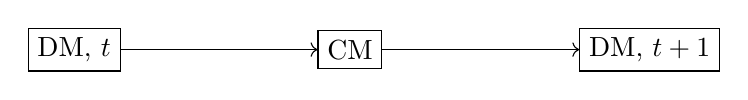
\begin{tikzpicture}[node distance=2.5cm]
        \node[draw, rectangle] (dm1) {DM, $t$};
        \node[draw, rectangle, right=of dm1] (cm) {CM};
        \node[draw, rectangle, right=of cm] (dm2) {DM, $t+1$};
        \draw[->] (dm1) -- (cm);
        \draw[->] (cm) -- (dm2);
    \end{tikzpicture}
    \end{center}
    \vspace{3mm}
    There are three nonstorable and perfectly divisible consumption goods at each date: fruit, general goods, and special goods. The only durable commodity in the economy is a set of ``Lucas trees''. The number of trees is fixed and equal to the number of agents. Trees yield fruit in the second subperiod of every period.
\end{frame}

\begin{frame}{Lagos}
    Each agent wishes to maximise
    \[
        \mathbb{E} \left\{ \sum_{t=0}^\infty \beta^t [u(q_t) - e(\tilde q_t) + v(y_t) + U(c_t) - A h_t]\right\}
    \]
    Where $\beta \in (0,1)$, $q_t$ and $\tilde q_t$ are the quantities of special goods consumed and produced in the decentralised market. $y_t$ denotes consumption of general goods, $c_t$ consumption of fruit, $h_t$ the number of hours worked in the second subperiod, and $\mathbb{E}$ is an expectations operator.

    Assume $u(0) = e(0) = 0$, $u' > 0$, $e' > 0$, $v' > 0$, $U' > 0$, $u'' < 0$, $e'' \ge 0$, $v'' \le 0$ and $U'' < 0$.
\end{frame}

\begin{frame}{Lagos}
    We begin by considering the case where the equity share is the only asset. Let $d_t$ be the quantity of fruit, or ``dividends'', produced by each tree in period $t$, and let $a_t$ be an individual agent's share holdings.
\end{frame}

\begin{frame}{Lagos}
    Let $W(a_t, d_t)$ denote the value function of an agent who enters the centralised market holding $a_t$ shares in a period where dividends are $d_t$, and let $V(a_t, d_t)$ denote the corresponding value function when he enters the decentralised market. These value functions satisfy the following Bellman equation:
    \[
        W(a_t, d_t) = \max_{c_t, y_t, n_t, h_t, a_{t+1}} \{U(c_t) + v(y_t) - A h_t + \beta \mathbb{E} V(a_{t+1}, d_{t+1})\}
    \]
    Subject to
    \[
        c_t + w_t n_t + \phi_t a_{t+1} = (\phi_t + d_t) a_t + w_t h_t
    \]
    \[
        0 \le c_t, \quad y_t = n_t, \quad 0 \le n_t, \quad 0 \le h_t \le \bar n, \quad 0 \le a_{t+1}
    \]
\end{frame}

\begin{frame}{Lagos}
    The agent chooses consumption of fruit ($c_t$), of general goods ($y_t$), how many hours of work to demand ($n_t$) and supply ($h_t$), and an end-of-period portfolio ($a_{t+1}$). Dividends $\{d_t\}$ follow a Markov process with $\mathbb{P}\{d_{t+1} \le x'| d_t = x\} = F(x', x)$. Fruit is used as numeraire: $w_t$ is the real wage, and $\phi_t$ the price of a share (ex-dividend).
\end{frame}

\begin{frame}{Lagos}
    Substituting the constraints that hold with equality,
    \[
        W(a_t, d_t) = \max_{c_t, n_t, a_{t+1}} \left\{ U(c_t) + v(n_t) - \frac{A}{w_t}[c_t + w_t n_t + \phi_t a_{t+1}] + \lambda_t a_t + \beta \mathbb{E} V(a_{t+1}, d_{t+1})\right\}
    \]
    Where $\lambda_t \equiv \frac{A}{w_t}(\phi_t + d_t)$.
\end{frame}

\begin{frame}{Lagos}
    Given the buyer and the seller have share holdings $a$ and $\tilde a$ respectively, the terms at which they trade in the decentralised market are $[q(a, \tilde a), p(a, \tilde a)]$, where $q(a, \tilde a) \in \mathbb{R}_+$ is the quantity of special good traded, and $p(a, \tilde a) \in \mathbb{R}_+$ represents the transfers of assets from the buyer to the seller. The value of an agent who enters the decentralised market with share holdings $a$ in a period when the dividend realisation is $d$, satisfies
    \begin{align*}
        V(a, d) &= \alpha \int \{u[q(a, \tilde a)] + W[a - p(a, \tilde a), d]\} dG(\tilde a) \\
        &\quad + \alpha \int \{-e[q(\tilde a, a)] + W[a + p(\tilde a, a), d]\} dG(\tilde a) + (1 - 2\alpha) W(a, d)
    \end{align*}
    where $G$ denotes the distribution of share holdings.
\end{frame}

\begin{frame}{Lagos}
    Consider a meeting in the decentralised market between a buyer holding $a_t$ and a seller holding $\tilde a_t$. The terms of trade $(q_t, p_t)$ are determined by Nash bargaining where the buyer has all the bargaining power:
    \[
        \max_{q_t, p_t \le a_t} \{u(q_t) + W(a_t - p_t, d_t) - W(a_t, d_t)\}
    \]
    Subject to
    \[
        -e(q_t) + W(\tilde a_t + p_t, d_t) \ge W(\tilde a_t, d_t)
    \]
    The constraint $p_t \le a_t$ indicates that the buyer cannot spend more assets than he owns.
\end{frame}

\begin{frame}{Lagos}
    Note that $W(a_t + p_t, d_t) - W(a_t, d_t) = \lambda_t p_t$, so the bargaining problem reduces to:
    \[
        \max_{q_t, p_t \le a_t} \{u(q_t) - \lambda_t p_t\}
    \]
    Subject to
    \[
        -e(q_t) + \lambda_t p_t \ge 0
    \]
    If $\lambda_t a_t \ge e(q^*)$ then the buyer exchanges $p_t = e(q^*)/\lambda_t \le a_t$ of his shares for the first-best quantity $q^*$. Else, he gives the seller all his shares, $p_t = a_t$, in exchange for the $q_t$ that solves $e(q_t) = \lambda_t a_t$. Note that the outcome depends only on $\lambda_t a_t$, and in particular, it is independent of the seller's asset holdings.
\end{frame}

\begin{frame}{Lagos}
    Hence, the solution to the bargaining problem is
    \[
        q(\lambda_t a_t) = \begin{cases} q^* & \text{if } \lambda_t a_t \ge e(q^*) \\ e^{-1}(\lambda_t a_t) & \text{if } \lambda_t a_t < e(q^*) \end{cases}
    \]
    Using this bargaining solution and the linearity of $W(a, d)$, the value of search can be written more compactly as
    \[
        V(a, d) = \mathcal{S}(\lambda a) + W(a, d)
    \]
    Where $\mathcal{S}(\lambda a) = \alpha \{u[q(\lambda a)] - e[q(\lambda a)]\}$. Observe that $\mathcal{S}$ is twice differentiable everywhere, with $\mathcal{S}' \ge 0$ and $\mathcal{S}'' \le 0$ (both inequalities are strict for $\lambda a < e(q^*)$).
\end{frame}

\begin{frame}{Lagos}
    Having characterised the terms of trade in decentralised exchange, we turn to the agent's individual optimisation problem in the centralised market.

    The agent's problem in the second subperiod is summarised by
    \begin{align*}
        W(a_t, d_t) &= \lambda_t a_t + \max_{c_t, n_t}\left\{ U(c_t) + v(n_t) - (c_t + w_t n_t) \frac{A}{w_t}\right\} \\
        &\quad + \max_{a_{t+1}}\left\{ \beta \mathbb{E} V(a_{t+1}, d_{t+1}) - \frac{A}{w_t} \phi_t a_{t+1}\right\}
    \end{align*}
\end{frame}

\begin{frame}{Lagos}
    Given that $U$ and $v$ are strictly concave, the unique solution $(c_t, n_t)$ satisfies
    \[
        U'(c_t) = \frac{A}{w_t}
    \]
    \[
        v'(n_t) = A
    \]
    The first-order condition for the choice of $a_{t+1}$ is
    \[
        \frac{A}{w_t} \phi_t = \beta \mathbb{E} V_a'(a_{t+1}, d_{t+1})
    \]
    From the DM value function we can show that
    \[
        V_a'(a_{t+1}, d_{t+1}) = \left[1 + \alpha\left( \frac{u'[q(\lambda_{t+1} a_{t+1})]}{e'[q(\lambda_{t+1} a_{t+1})]} - 1\right)\right] \lambda_{t+1}
    \]
\end{frame}

\begin{frame}{Lagos}
    Note that none of the agent's choices depend on his individual asset holdings. We will consider an equilibrium in which all prices are time-invariant function of the aggregate state: $w_t = w(d_t)$, $\phi_t = \phi(d_t)$, and therefore, $\lambda_t = \lambda(d_t) \equiv \frac{A}{w(d_t)}[\phi(d_t) + d_t]$.
\end{frame}

\begin{frame}{Lagos}
    A \emph{recursive equilibrium} is a collection of individual decision rules $c_t = c(d_t)$, $n_t = n(d_t)$, $a_{t+1} = a(d_t)$, pricing functions $w_t = w(d_t)$ and $\phi_t = \phi(d_t)$ and bilateral terms of trade $q_t = q(d_t)$ and $p_t = p(d_t)$ such that:
    \begin{enumerate}[(a)]
        \item The decision rules $c(\cdot)$, $n(\cdot)$, and $a(\cdot)$, solve the agent's problem in the decentralised market, given prices
        \item The terms of trade are determined by Nash bargaining, i.e., $q[\lambda(d_t) a_t]$ and $p(d_t) = \min\left[a_t, \frac{e(q^*)}{\lambda(d_t)}\right]$; and
        \item Prices are such that the centralised market clears, i.e., $c(d_t) = d_t$, and $a(d_t) = 1$.
    \end{enumerate}
\end{frame}

\section{Adding a Bond}

\begin{frame}{Lagos}
    In this section, we introduce a government-issued one-period risk-free real bill, which we will refer to as a ``bond''. Let $B_t$ denote the stock of bonds that are outstanding in period $t$, to be redeemed before the centralised trading session of period $t$. (The government sells $B_{t+1}$ in the centralised market at the end of period $t$). What we call the ``government'', is essentially summarised by the budget constraint
    \[
        B_t = \phi^b_t B_{t+1} + \tau_t
    \]
    Where $\phi^b_t$ is the price of a bond, and $\tau_t$ a lump-sum tax levied on all agents during the centralised trading session, both expressed in terms of fruit.
\end{frame}

\begin{frame}{Lagos}
    The focus here is not on how the government should select the path $\{B_t, \tau_t\}$, but rather on characterising the equilibrium, and in particular asset prices and return, given such a path. Let $\mathbf{a}_t \in \mathbb{R}^2_+$ denote an agent's portfolio. Since they can now hold two assets, $\mathbf{a}_t = \{a^s_t, a^b_t\}$, where $a^s_t$ and $a^b_t$ denote the holdings of shares and bonds, respectively. Let $\phi^s_t$ be the price of s share in terms of fruit, and $\boldsymbol{\phi}_t = \{\phi^s_t, \phi^b_t\}$.
\end{frame}

\begin{frame}{Lagos}
    The value function of an agent who enters the centralised market with portfolio $\mathbf{a}_t$ in a period when dividends are $d_t$ now satisfies:
    \[
        W(\mathbf{a}_t, d_t) = \max_{c_t, n_t, h_t, \mathbf{a}_{t+1}} \{U(c_t) + v(n_t) - A h_t + \beta \mathbb{E} V(\mathbf{a}_{t+1}, d_{t+1})\}
    \]
    Subject to
    \[
        c_t + w_t n_t + \boldsymbol{\phi}_t \mathbf{a}_{t+1} = (\phi^s_t + d_t) a^s_t + a^b_t + w_t h_t - \tau_t
    \]
    \[
        0 \le c_t, \quad 0 \le n_t, \quad 0 \le h_t \le \bar n, \quad 0 \le \mathbf{a}_{t+1}
    \]
\end{frame}

\begin{frame}{Lagos}
    In the decentralised market, the terms at which a buyer with portfolio $\mathbf{a}$ trades with a seller with portfolio $\tilde{\mathbf{a}}$ are $[q(\mathbf{a}, \tilde{\mathbf{a}}), \mathbf{p}(\mathbf{a}, \tilde{\mathbf{a}})]$, where $q(\mathbf{a}, \tilde{\mathbf{a}}) \in \mathbb{R}_+$ is the quantity of special good traded, and $\mathbf{p}(\mathbf{a}, \tilde{\mathbf{a}}) \in \mathbb{R}^2_+$ represents the transfer of assets from the buyer to the seller.

    The value of an agent who enters the decentralised market holding portfolio $\mathbf{a}$ in a period when the dividend realisation is $x$, satisfies
    \begin{align*}
        V(\mathbf{a}, x) &= \alpha \int \{u[q(\mathbf{a}, \tilde{\mathbf{a}})] + W[\mathbf{a} - \mathbf{p}(\mathbf{a}, \tilde{\mathbf{a}}), x]\} d\mathbf{G}(\tilde{\mathbf{a}}) \\
        &\quad + \alpha \int \{-e[q(\tilde{\mathbf{a}}, \mathbf{a})] + W[\mathbf{a} + \mathbf{p}(\tilde{\mathbf{a}}, \mathbf{a}), x]\} d\mathbf{G}(\tilde{\mathbf{a}}) + (1 - 2\alpha) W(\mathbf{a}, x)
    \end{align*}
    Where $\mathbf{G}$ denotes the distribution of portfolios.
\end{frame}

\begin{frame}{Lagos}
    The terms of trade $[q(\mathbf{a}, \tilde{\mathbf{a}}), \mathbf{p}(\mathbf{a}, \tilde{\mathbf{a}})]$ are still determined by Nash bargaining where the buyer has all the bargaining power:
    \[
        \max_{q_t, \mathbf{p}_t \le \mathbf{a}_t} \{u(q_t) + W(\mathbf{a}_t - \mathbf{p}_t, d_t) - W(\mathbf{a}_t, d_t)\}
    \]
    Subject to
    \[
        -e(q_t) + W(\tilde{\mathbf{a}} + \mathbf{p}_t, d_t) \ge W(\tilde{\mathbf{a}}, d_t)
    \]
    Let $\lambda^b_t = \frac{A}{w_t}$, $\lambda^s_t = \frac{A}{w_t}(\phi^s_t + d_t)$, and note that $W(\mathbf{a}_t + \mathbf{p}_t, d_t) - W(\mathbf{a}_t, d_t) = \boldsymbol{\lambda}_t \mathbf{p}_t$, where $\boldsymbol{\lambda}_t = \{\lambda^s_t, \lambda^b_t\}$.
\end{frame}

\begin{frame}{Lagos}
    These observations imply that the bargaining problem reduces to
    \[
        \max_{q_t, \mathbf{p}_t \le \mathbf{a}_t} \{u(q_t) - \boldsymbol{\lambda}_t \mathbf{p}_t\}
    \]
    Subject to
    \[
        -e(q_t) + \boldsymbol{\lambda}_t \mathbf{p}_t \ge 0
    \]
    The solution is $q(\boldsymbol{\lambda}_t \mathbf{a}_t)$, where the function $q(\cdot)$ is still given by
    \[
        q(\boldsymbol{\lambda}_t \mathbf{a}_t) = \begin{cases} q^* & \text{if } \boldsymbol{\lambda}_t \mathbf{a}_t \ge e(q^*) \\ e^{-1}(\boldsymbol{\lambda}_t \mathbf{a}_t) & \text{if } \boldsymbol{\lambda}_t \mathbf{a}_t < e(q^*) \end{cases}
    \]
\end{frame}

\begin{frame}{Lagos}
    Using the bargaining solution and the fact that $W[\mathbf{a} + \mathbf{p}(\mathbf{a}, \tilde{\mathbf{a}}), d] - W(\mathbf{a}, d) = \boldsymbol{\lambda}_t \mathbf{p}(\mathbf{a}, \tilde{\mathbf{a}})$, the value of search can be written as:
    \[
        V(\mathbf{a}, d) = \sum_{i=1}^2 \theta_i \mathcal{S}(\boldsymbol{\lambda}^i \mathbf{a}) + W(\mathbf{a}, d)
    \]
    In the centralised market, the agent's choices of $c_t$ and $n_t$ are still characterised by
    \[
        U'(c_t) = \frac{A}{w_t}
    \]
    \[
        v'(n_t) = A
    \]
\end{frame}

\begin{frame}{Lagos}
    The first-order conditions for asset holdings, $\mathbf{a}_{t+1}$ are
    \[
        \frac{A}{w_t} \phi^i_t = \beta \mathbb{E} \frac{dV(\mathbf{a}_{t+1}, d_{t+1})}{d a^i_{t+1}}, \quad i = s, b
    \]
    Where
    \begin{align*}
        \frac{dV(\mathbf{a}_{t+1}, d_{t+1})}{d a^b_{t+1}} &= \left[ 1 + \alpha \sum_{i=1}^2 \theta_i \left( \frac{u'[q(\boldsymbol{\lambda}^i_{t+1} \mathbf{a}_{t+1})]}{e'[q(\boldsymbol{\lambda}^i_{t+1} \mathbf{a}_{t+1})]} - 1 \right)\right] \lambda^b_{t+1} \\
        \frac{dV(\mathbf{a}_{t+1}, d_{t+1})}{d a^s_{t+1}} &= \left[ 1 + \alpha \theta_2 \left( \frac{u'[q(\boldsymbol{\lambda}^2_{t+1} \mathbf{a}_{t+1})]}{e'[q(\boldsymbol{\lambda}^2_{t+1} \mathbf{a}_{t+1})]} - 1\right)\right] \lambda^s_{t+1}
    \end{align*}
    As usual, the agent's choices do not depend on his individual asset holdings, and the distribution of assets will be degenerate in equilibrium.
\end{frame}

\begin{frame}{Lagos}
    Given the dividend process $\{d_t\}_{t=0}^\infty$ and a path $\{B_t, \tau_t\}_{t=0}^\infty$, an equilibrium is an allocation $\{c_t, n_t, \mathbf{a}_{t+1}\}_{t=0}^\infty$ together with the set prices $\{w_t, \boldsymbol{\phi}_t\}_{t=0}^\infty$ and bilateral terms of trade $\{q_t\}_{t=0}^\infty$, such that:
    \begin{enumerate}[(a)]
        \item The individual choices $\{c_t, n_t, \mathbf{a}_{t+1}\}_{t=0}^\infty$ solve the agent's problem in the decentralised market, given prices;
        \item The terms of trade are determined by Nash bargaining, i.e.,
        \[
            q^1_t = \min \left\{ q^*, e^{-1} \left( \frac{A}{w_t} a^b_t\right)\right\} \text{ and } q^2_t = \min \left\{ q^*, e^{-1} \left[ \frac{A}{w_t}(\phi^s_t + d_t) a^s_t + \frac{A}{w_t} a^b_t\right]\right\}
        \]
        \item Prices are such that the centralised market clears, i.e., $c_t = d_t$, $a^s_{t+1} = 1$, and $a^b_{t+1} = B_{t+1}$.
    \end{enumerate}
\end{frame}

\section{Asset Pricing}

\begin{frame}{Lagos}
    In a recursive equilibrium, allocations and prices are time-invariant of the aggregate state $x$, the current dividend realisation. Specifically, $\phi^s_t = \phi^s(x_t)$, $\phi^b_t = \phi^b(x_t)$ and $w_t = w(x_t) \equiv \frac{A}{U'(x_t)}$. In addition, $\lambda^s_t = \lambda^s(x_t) \equiv U'(x_t)[\phi^s(x_t) + x_t]$, and $\lambda^b_t = U'(x_t)$. Also, suppose that the government follows the stationary policy $B_{t+1} = B(x_t)$, and that the aggregate state follows a Markov process with $\mathbb{P}\{x_{t+1} \le x'| x_t = x\} = F(x', x)$.
\end{frame}

\begin{frame}{Lagos}
    Then, asset prices satisfy:
    \[
        \lambda^s(x) - U'(x) x = \beta \int L^s(x') \lambda^s(x') dF(x', x)
    \]
    \[
        U'(x) \phi^b(x) = \beta \int L^b(x') U'(x') dF(x', x)
    \]
    Where
    \[
        L^s(x') = 1 + \alpha(1-\theta) \left( \frac{u'\{q[\lambda^s(x') + U'(x') B']\}}{e'\{q[\lambda^s(x') + U'(x') B']\}} - 1\right)
    \]
    $B' = B(x)$, and
    \[
        L^b(x') = L^s(x') + \alpha \theta \left( \frac{u'\{q[U'(x') B']\}}{e'\{q[U'(x') B']\}} - 1\right)
    \]
    To simplify notation, we have set $\theta_1 = \theta$.
\end{frame}

\begin{frame}{Lagos}
    \textbf{The Equity Premium and Risk-Free Rate Puzzles}

    Use the \emph{intrinsic returns} $\hat R^b(x)$ and $\hat R^s(x, x')$, to define the \emph{full returns} $R^b(x, x') = L^b(x') \hat R^b(x)$, and $R^s(x, x') = L^s(x') \hat R^s(x, x')$ and write the asset prices as
    \[
        \int \beta \frac{U'(x')}{U'(x)} R^i(x, x') dF(x', x) = 1
    \]
    for $i = s, b$ and all $x$.
\end{frame}

\begin{frame}{Lagos}
    Let $\bar F$ be the invariant distribution for the transition function $F$; then the Euler equations lead to:
    \[
        \int \int \beta \frac{U'(x')}{U'(x)} [R^s(x, x') - R^b(x, x')] dF(x', x) d\bar F(x) = 0
    \]
    \[
        \int \int \beta \frac{U'(x')}{U'(x)} R^b(x, x') dF(x', x) d\bar F(x) - 1 = 0
    \]
    a pair of statistical restrictions on equilibrium asset returns $R^i(x, x')$, and the marginal rate of substitution, $\beta \frac{U'(x')}{U'(x)}$.
\end{frame}

\begin{frame}{Lagos}
    For the special case of an economy with no liquidity needs (i.e., $\alpha = 0$), the intrinsic returns equal the full returns, i.e., $\hat R^s(x, x') = R^s(x, x')$ and $\hat R^b(x) = R^b(x, x')$. In this case, one can estimate the expectations of the left hand sides of the Euler equations using the sample means
    \[
        \hat \omega^e = \frac{1}{T} \sum_{t=1}^T \beta \frac{U'(c_{t+1})}{U'(c_t)} [\hat R^s_{t+1} - \hat R^b_t]
    \]
    \[
        \hat \omega^b = \frac{1}{T} \sum_{t=1}^T \beta \frac{U'(c_{t+1})}{U'(c_t)} \hat R^b_t - 1
    \]
    A vast body of work has been devoted to trying to rationalise the finding that for standard parameterisation of preferences, the statistical restrictions $\hat \omega^e = \hat \omega^b = 0$ are violated by U.S. data. The finding that $\hat \omega^e > 0$ constitutes the \textcolor{blue}{equity premium puzzle}, while $\hat \omega^b < 0$ is referred to as the \textcolor{blue}{risk-free rate puzzle}.
\end{frame}

\begin{frame}{Lagos}
    The statistics $\hat \omega^e$ and $\hat \omega^b$ that define these puzzles are constructed using only the \emph{intrinsic returns}, $\hat R^s_{t+1}$ and $\hat R^b_t$. But according to the model that we have developed, agents price assets using the \emph{full returns} $R^s_{t+1}$ and $R^b_{t+1}$, that is, the intrinsic returns augmented by their respective liquidity factors.
\end{frame}

\begin{frame}{Lagos}
    In our case we can write
    \[
        \int \int \beta \frac{U'(x')}{U'(x)} [\hat R^s(x, x') - \hat R^b(x, x')] dF(x', x) d\bar F(x) = \omega^e
    \]
    \[
        \int \int \beta \frac{U'(x')}{U'(x)} \hat R^b(x, x') dF(x', x) d\bar F(x) - 1 = \omega^b
    \]
    Where
    \[
        \omega^e = \int \int \beta \frac{U'(x')}{U'(x)} \left\{ [L^b(x') - 1] \hat R^b(x) - [L^s(x') - 1] \hat R^s(x, x')\right\} dF(x, x') d\bar F(x)
    \]
    \[
        \omega^b = -\int \int \beta \frac{U'(x')}{U(x)} [L^b(x') - 1] \hat R^b(x) dF(x, x') d\bar F(x)
    \]
\end{frame}

\begin{frame}{Lagos}
    Note that $\omega^e$ and $\omega^b$ are the theoretical counterparts to $\hat \omega^e$ and $\hat \omega^b$, respectively. The left hand side of the first Euler equation is a weighted average of the excess intrinsic return of equity over bonds, which in equilibrium must equal $\omega^e$. The wedge $\omega^e$ will be larger, the larger $\frac{L^b - 1}{L^s - 1} - \frac{\hat R^s}{\hat R^b}$ is on average, i.e., the larger is the excess liquidity return of bonds over equity relative to the excess intrinsic return of equity over bonds.
\end{frame}

\begin{frame}{Lagos}
    The sign of $\omega^e$ is ambiguous in general. But to the extent that bonds are more liquid than equity (in the sense of larger $\theta$), the latter will tend to pay an ``illiquidity premium'', implying $\omega^e > 0$. Note that even without assuming any exogenous liquidity differences between equity and bonds, we have $\omega^b < 0$, to the extent that there are liquidity needs at least for some realisations of the dividend process. Thus, qualitatively, the model with liquidity needs is always consistent with the risk-free rate puzzle. And in addition, if the liquidity return on bonds is large enough relative to that on equity, then the model may also help rationalise the equity premium puzzle.
\end{frame}

\begin{frame}[allowframebreaks]{References}
    \small
    \begin{thebibliography}{99}
        \bibitem[Lagos(2010)]{lagos2010}
            Lagos, R.\ Asset prices and liquidity in an exchange economy. \textit{Journal of Monetary Economics}, 57(8):913--930, 2010.
    \end{thebibliography}
\end{frame}

\end{document}
